\section{Referencia de la Clase listlinpresupuestoview}
\label{classlistlinpresupuestoview}\index{listlinpresupuestoview@{listlinpresupuestoview}}
Muestra y administra el detalle de las l\'{\i}neas de un presupuesto.  


{\tt \#include $<$listlinpresupuestoview.h$>$}

Diagrama de herencias de listlinpresupuestoview\begin{figure}[H]
\begin{center}
\leavevmode
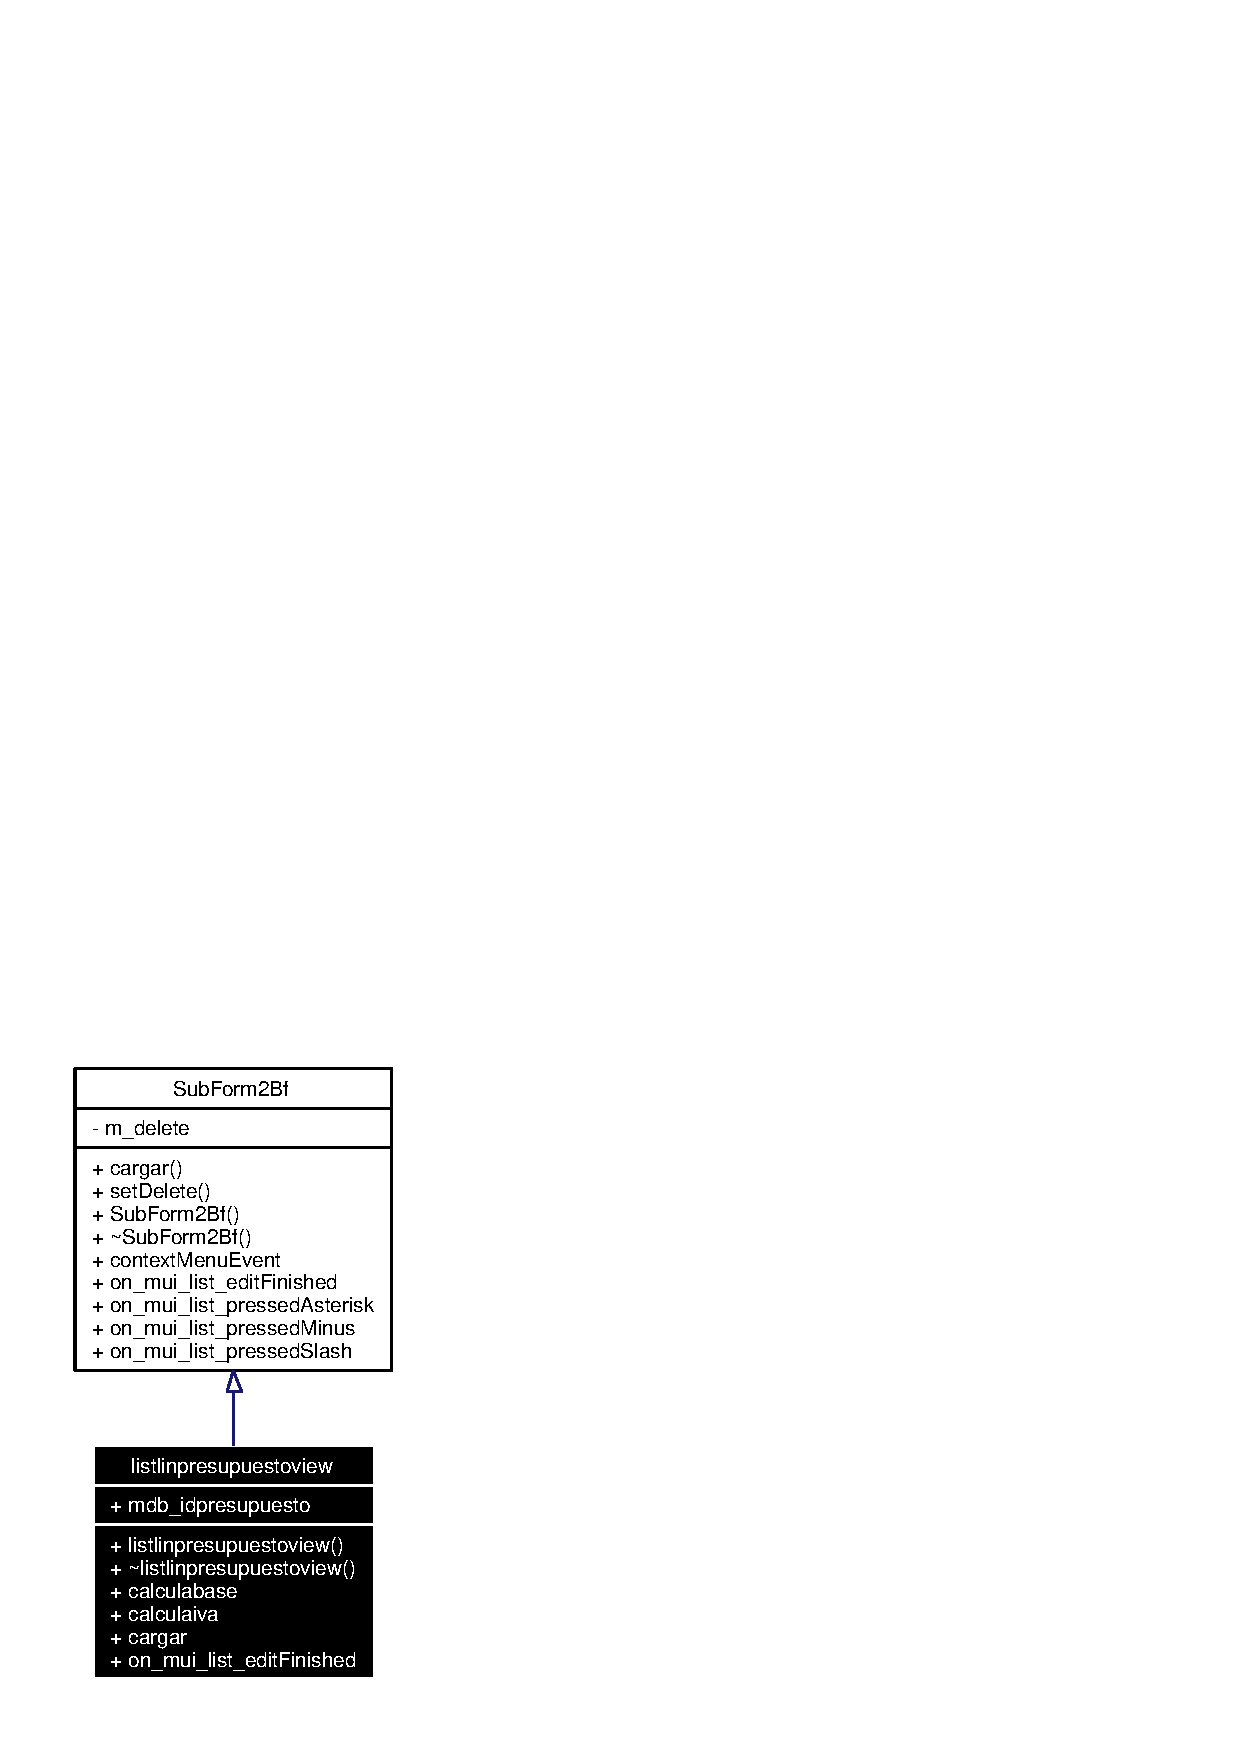
\includegraphics[width=94pt]{classlistlinpresupuestoview__inherit__graph}
\end{center}
\end{figure}
Diagrama de colaboraci\'{o}n para listlinpresupuestoview:\begin{figure}[H]
\begin{center}
\leavevmode
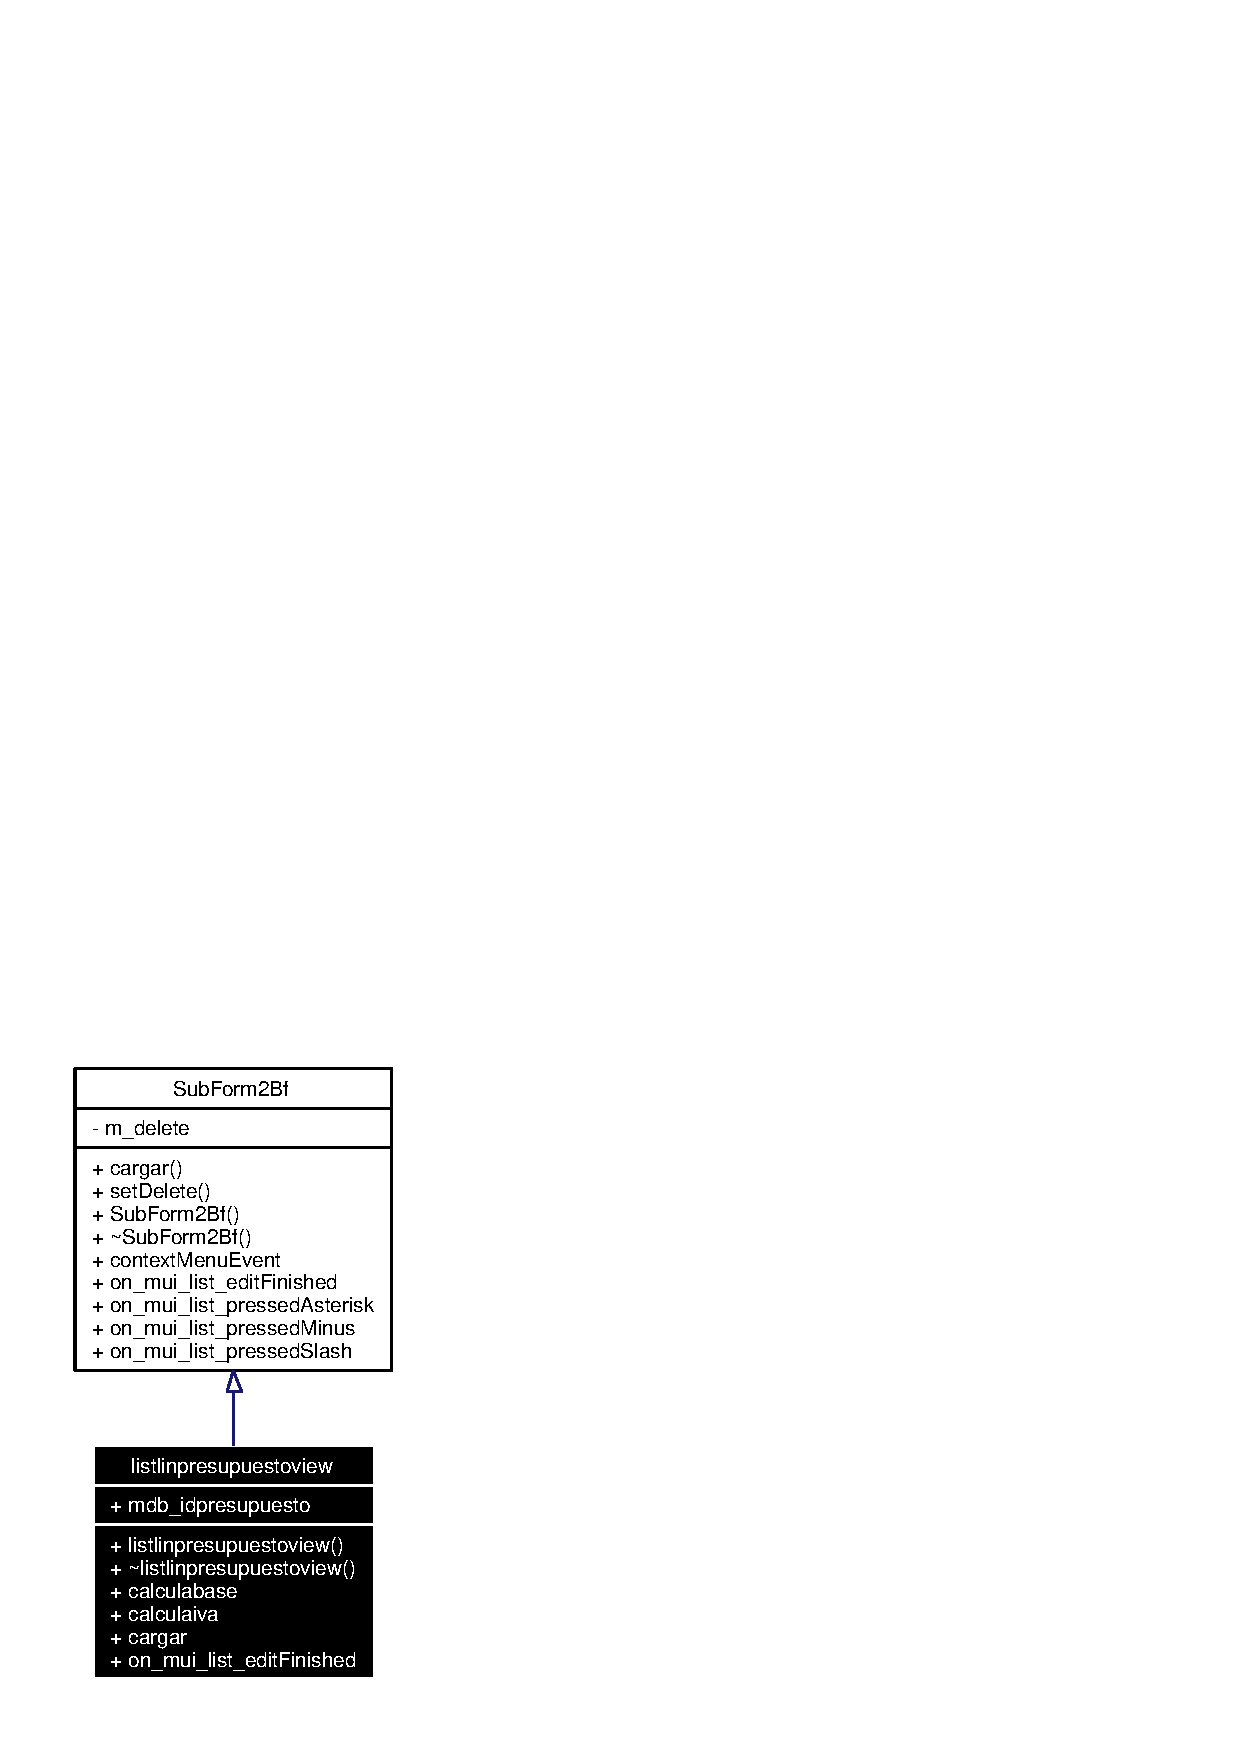
\includegraphics[width=94pt]{classlistlinpresupuestoview__coll__graph}
\end{center}
\end{figure}
\subsection*{Slots p\'{u}blicos}
\begin{CompactItemize}
\item 
Fixed {\bf calculabase} ()\label{classlistlinpresupuestoview_i0}

\item 
Fixed {\bf calculaiva} ()\label{classlistlinpresupuestoview_i1}

\item 
virtual void {\bf cargar} (QString idpresupuesto)\label{classlistlinpresupuestoview_i2}

\item 
virtual void {\bf on\_\-mui\_\-list\_\-edit\-Finished} (int, int)\label{classlistlinpresupuestoview_i3}

\end{CompactItemize}
\subsection*{M\'{e}todos p\'{u}blicos}
\begin{CompactItemize}
\item 
{\bf listlinpresupuestoview} (QWidget $\ast$parent=0)\label{classlistlinpresupuestoview_a0}

\end{CompactItemize}
\subsection*{Atributos p\'{u}blicos}
\begin{CompactItemize}
\item 
QString {\bf mdb\_\-idpresupuesto}\label{classlistlinpresupuestoview_o0}

\end{CompactItemize}


\subsection{Descripci\'{o}n detallada}
Muestra y administra el detalle de las l\'{\i}neas de un presupuesto. 



La documentaci\'{o}n para esta clase fu\'{e} generada a partir de los siguientes archivos:\begin{CompactItemize}
\item 
listlinpresupuestoview.h\item 
listlinpresupuestoview.cpp\end{CompactItemize}
